\chapter{Výsledky studentské práce}

% Referenční skladby http://isophonics.net/about

\section{Výběr vhodných metod pro extrakci vlastností hudební nahrávky} \label{sec:Exktrakce_vlastnosti_metody}

Vědeská komunita nabízí několik volně šířících knihoven obsahující techniky z oborů MIR. V této části práce jsou prozkoumány 3 knihovny zmíněné v bodě \ref{sec:Dostupna_reseni}. Jsou použity jejich funkce získání potřebných parametrů hudební nahrávky potřebných pro navazující diplomovou práci. Tyto funkce jsou mezi sebou porovnány z hlediska přesnosti výsledků, rychlosti výpočtů, jednoduchosti použití a možnosti využití pro komerční účely. 

\subsection{Detekce dob a tempa}



\subsection{Analýza chromavektorů}



\section{Návrh výsledného systému}

Návrh popisuje komplexní systém skládající se z několika částí, uživatelské rozhraní algoritmů pro získání pamrametrů hudební nahrávky a algoritmu generujícího SpectodaCode na základě získaných parametrů. V této kapitole je podrobně popsán návrh jednotlivých částí systému. 

\subsection{Uživatelské rozhraní}

Uživatelské rozhraní je reprezentováno webovou stránkou a je naprogramováno pomocí značkovacího jazyka \acs{HTML} spolu s formátováním v jazyce CSS. Funkčnosto webové stránky je zajištěna funkcemi jazyce JavaScript. Javascript také vytváří propojovací můstek pro komunikaci s vnistřním systémem v jazyce Python.

Jedná se o jednoduché webové rozhraní ve kterém uživatel nahraje hudební skladbu ve formátu .wav. Rozhranní obsahuje pole pro vložení cesty k hudební skladbě umožňující výběr ze souborů v uživatelově uložišti, 4 tlačítka pro výběr nálady
\uv{mood}. Jedná se o tlačítka: \uv{chill}, \uv{feeling happy}, \uv{hang out} a \uv{dancing}. Pod tlačítky pro výběr nálady se nachází tlačítko pro spuštění procesu generování SpectodaCodu.
 Poslední částí webového rozhraní je textové pole ve kterém se zobrazí vygenerovaný SpectodaCode.

% TODO Jednoduché blokové schéma postupu uživatele od otevření stránky k získání kódu.

Na blokovém schématu výše je zobrazen proces postupu uživatele skrze webové rozhraní. 

\subsection{Parametry hudební nahrávky} \label{sec:Parametry_nahravky}

Systém popsaný v bodě \ref{sec:System_generovani_animaci} vyžaduje vstupní data o hudební nahrávce. Tyto data jsou rozdělena 7 odlišných objektů. Každý z těchto objektů představuje určitou vlastnost analyzované nahrávky. Tyto vlastnosti jsou získány pomocí technik popsaných v bodě \ref{sec:Exktrakce_vlastnosti_metody}. Jednotlivé vlastnosti a jejich datové struktury jsou shrnuty v následujících bodech.

\begin{description}
    \item[Detekce dob] představuje pole hodnot jehož délka je závislá na době trvání nahrávky. Jednotlivé hodnoty pak udávají časy hudební nahrávky, ve kterých se nacházejí doby. %TODO: Obrázek
    \item[Tempo skladby] je číslo typu float s jednotkou \acs{BPM} vyjadřující počet úderů za minutu. Hodnota BPM se vztahuje k počtu čtvrťových not za minutu. Vybraný algoritmus s knihovny Librosa ovšem nedetekuje jestli se jedná o noty čtvrťové. Postup zjištění tempa je popsán v bodě \ref{Librosa}.
    \item[Chromavektory] jsou získány v podobě pole jehož počet řádků udává 12 půltónů rozdělujících 1 oktávu. Délka pole je závislá na délce nahrávky a velikosti okna  při výpočtu \acs{STFT}. K matici chromavektorů je přidáno pole o stejné délce. Hondonty v poli udávají čas konce okna, ve kterém jsou počítány chroma vlastonsti. Tyto dvě proměnné jsou zadány jako parametry třídy s názvem $ChromaVector$ jehož struktura je zobrazena v blokovém schématu \ref{fig:ChromaVector_class_diagram}.

    \begin{figure}[H]
        \centering
        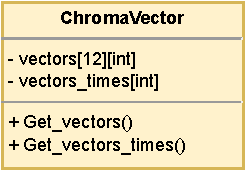
\includegraphics[width = 0.3\linewidth]{obrazky/UML_diagram_ChromaVector.pdf}
        \caption{Struktura třídy $ChromaVector$}
        \label{fig:ChromaVector_class_diagram}
    \end{figure}

    \item[Efektivní hodnota signálu] je zapsána třídou $Loudness$ obsahující dva atributy. Prvním z nich je pole $rms$ jehož délka je závislá na délce signálu a obsahuje efektivní hodnoty signálu v časech uložených v druhém atributu. Druhý atribut $times$ je pole o stéjné délce jako pole s hodnoty rms a obsahuje časy skladby ve kterých je hodnota rms počítána. 
    
    \begin{figure}[H]
        \centering
        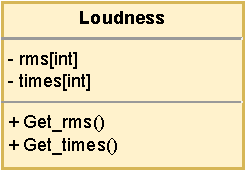
\includegraphics[width = 0.3\linewidth]{obrazky/UML_diagram_Loudness.pdf}
        \caption{Struktura třídy $Loudness$}
        \label{fig:Loudness_class_diagram}
    \end{figure}

    \item[Segmentace] je zapsána jako pole objektů tířdy $Segment$. Tato třída obshahuje 3 atributy $type$, $start\_time$ a $end\_time$. Argument $type$ obsahuje statickou hodnotu označující o jakou část skladby se jedná. Tyto hodnoty jsou vypsány v úryvku kódu.... %TODO: sepsat statické hodnoty.
    Argumenty $start\_time$ a $end\_time$ označují začátek a konec segmentu v nahrávce. 

    \begin{figure}[H]
        \centering
        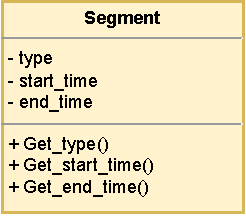
\includegraphics[width = 0.3\linewidth]{obrazky/UML_diagram_Segment.pdf}
        \caption{Struktura třídy $Segment$}
        \label{fig:Loudness_Segment_diagram}
    \end{figure}

    \item[Žánr] představuju proměnou typu short vekteré je zapsáno číslo označující žánr skladby. Statické hodnoty žánrů jsou zapsány v úryvku kódu .... %TODO: doplnit statické typy žánrů.
    \item[Nálada] stejně jako žánr představuje proměno typu short s přednastavenými statickými hodnotami zobrazenými v části kódu ... %TODO: doplnit statické typy žánrů.
\end{description}

\subsection{Systém pro generování animací} \label{sec:System_generovani_animaci}

Vstupními parametry systému jsou získané parametry jež jsou popsány v bodě \ref{sec:Parametry_nahravky} 

% Možná lepší první popsat strukturu systému jak by se měly animace generovat a co k tomu budou potřeba za parametry. Následně teprve vytvořit sekci kde je popsán vzniklý kód pro analýzu jednotlivých parametrů. Také důležité jestli ukázaky kódu atd.. nebudou zahrnuty spíše v sekci Věběr vhodných metod pro extrakci vlastností hudební nahrávky. 